\documentclass{article}

\usepackage{Sweave}
\begin{document}
\Sconcordance{concordance:prief_outline.tex:prief_outline.Rnw:%
1 2 1 1 0 47 1}


\section{Framing}
\begin{enumerate}
\item Focus on SPE's. We think they matter but we can't, tell in the long term because of covariation with germination percentage. Use emprical data to show that similar species have different phenological responses to temperature, but their germination fractions differ too. Use our models to isolate priorty effects (only bring the runs where both species germinate to the same fraction)
\item Lead w/ SPE's. Set up that these are dictated by temperature. But, they aren't the only aspect of germination that is...fraction is too. Or just introduce the idea multple aspects of germination are controlled by environment. They covary (see emprical data). They have similar within year implications (greater diffs result in more biomass for earlier/larger fraction). Different across year ( ie storage effect for germ \% repeated bad years followed by a good year year means super good, but phenology doesn't work that way. Thus climate change might affect the coexistence/competions trade offs differently. Climate change: When chilling is high, chilling is met, so sensitivity differences manifest in smaller realized differences in phenolgoy and fraction, so Rstar really dominates the interaction. when chilling goes down, sensitivity differences generate more pronounced realized pheno fract differences so the shape of the tradeoff changes.)
\end{enumerate}


\begin{figure}[h!]
  \centering
 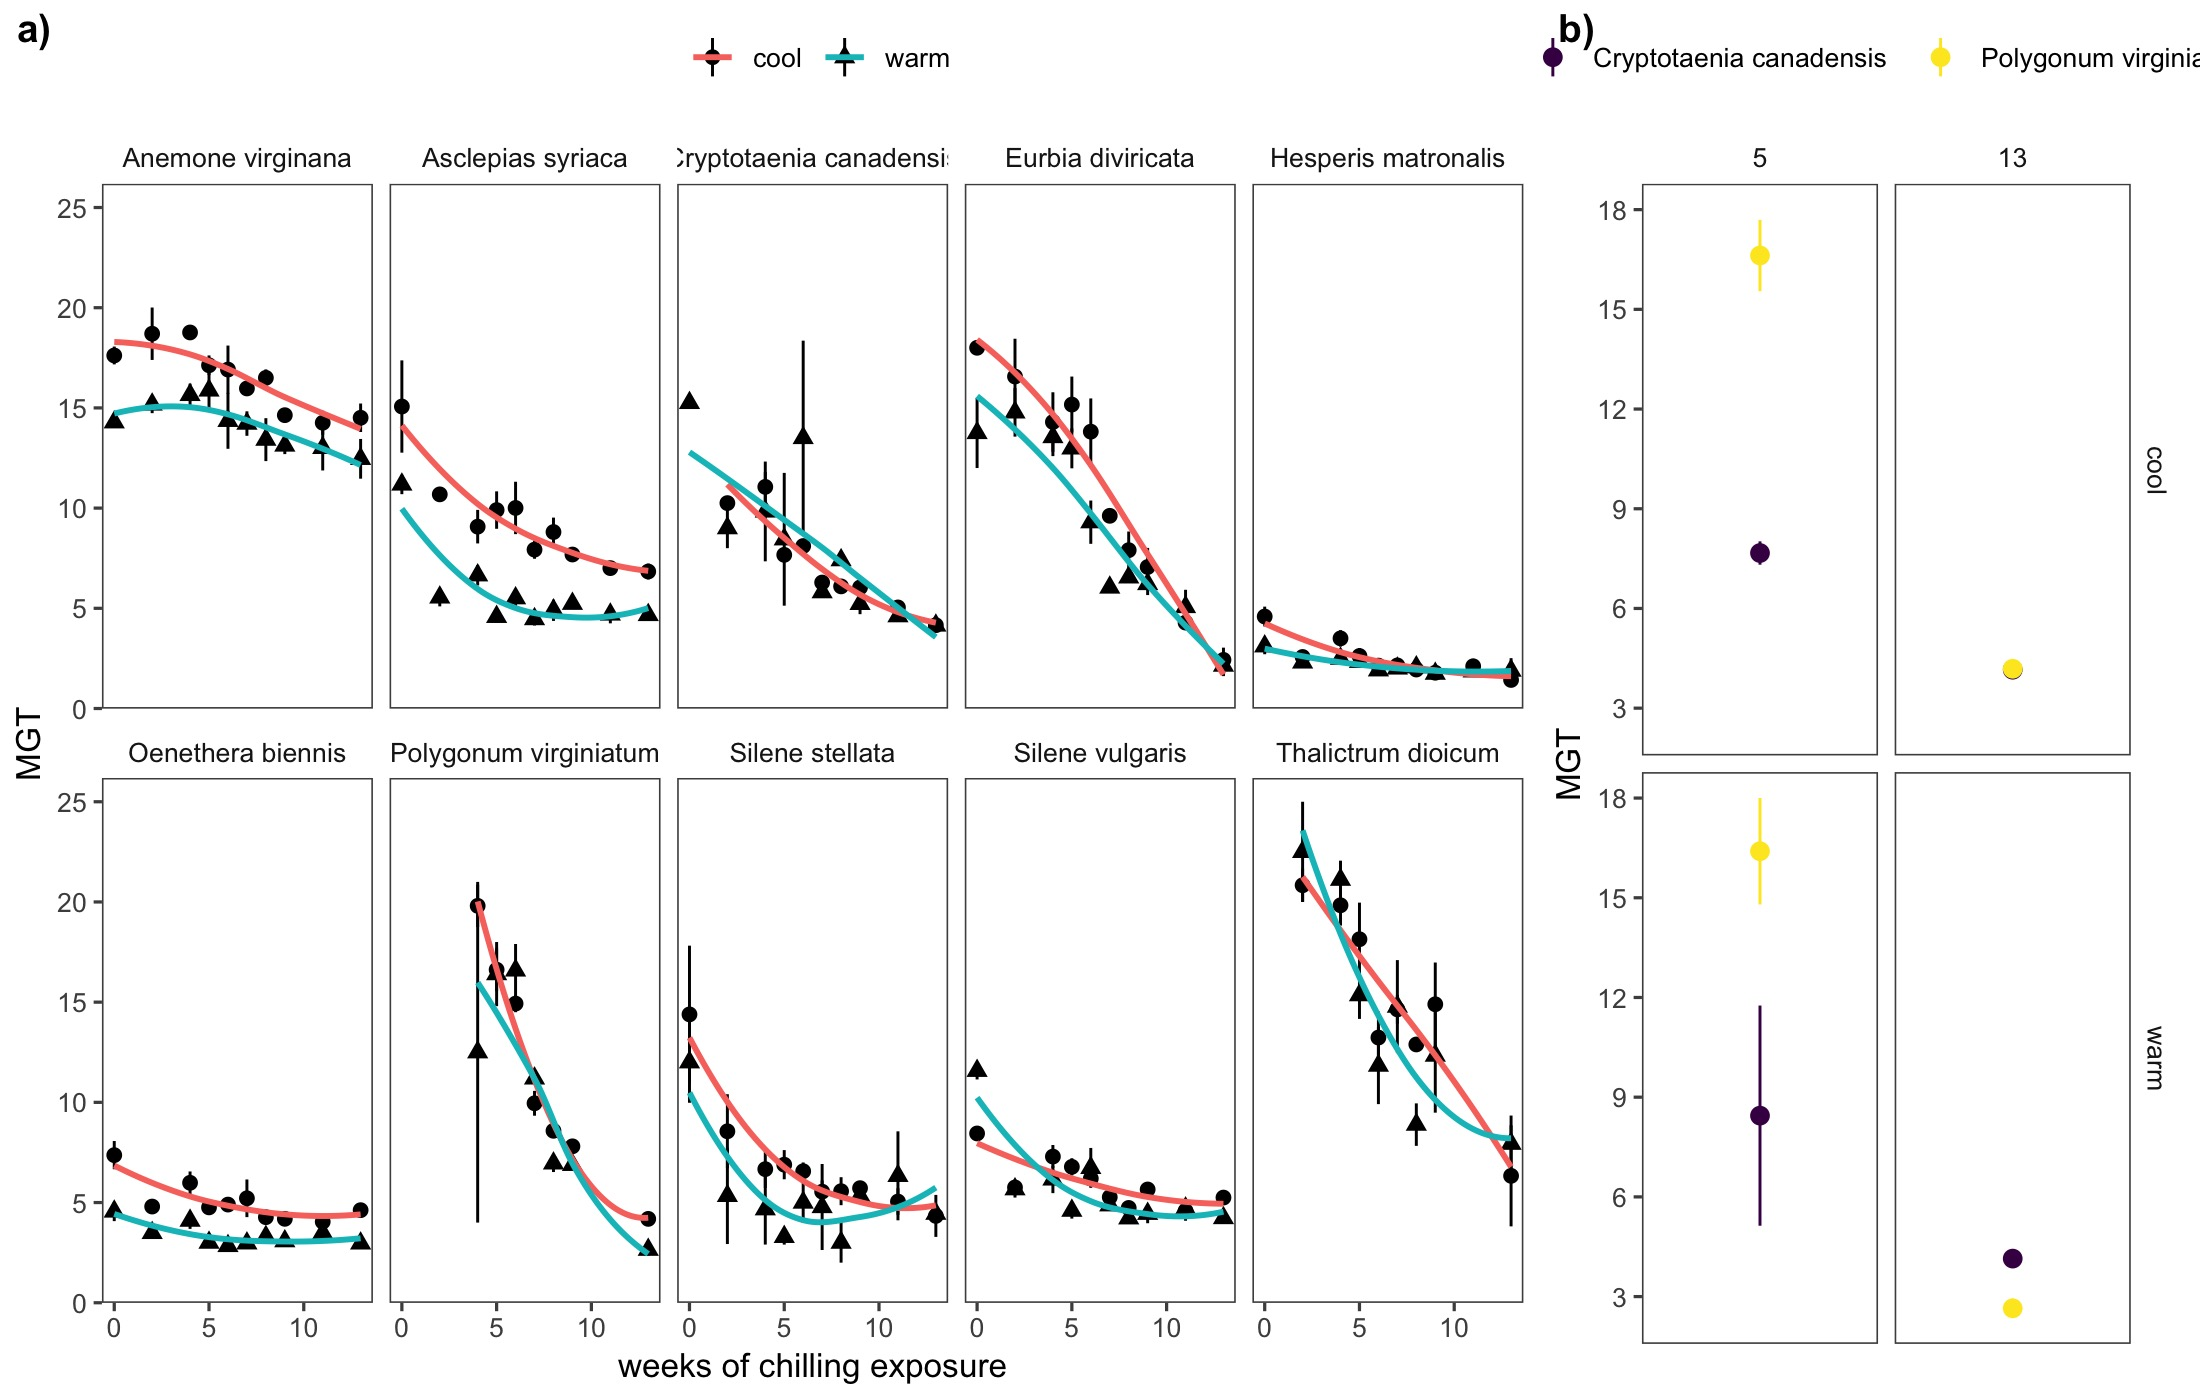
\includegraphics[width=\textwidth]{..//plots/empricalplots2.jpeg}
    \caption{potential empirical plot style?}
    \label{Fig:emp}
\end{figure}

\begin{figure}[h!]
  \centering
 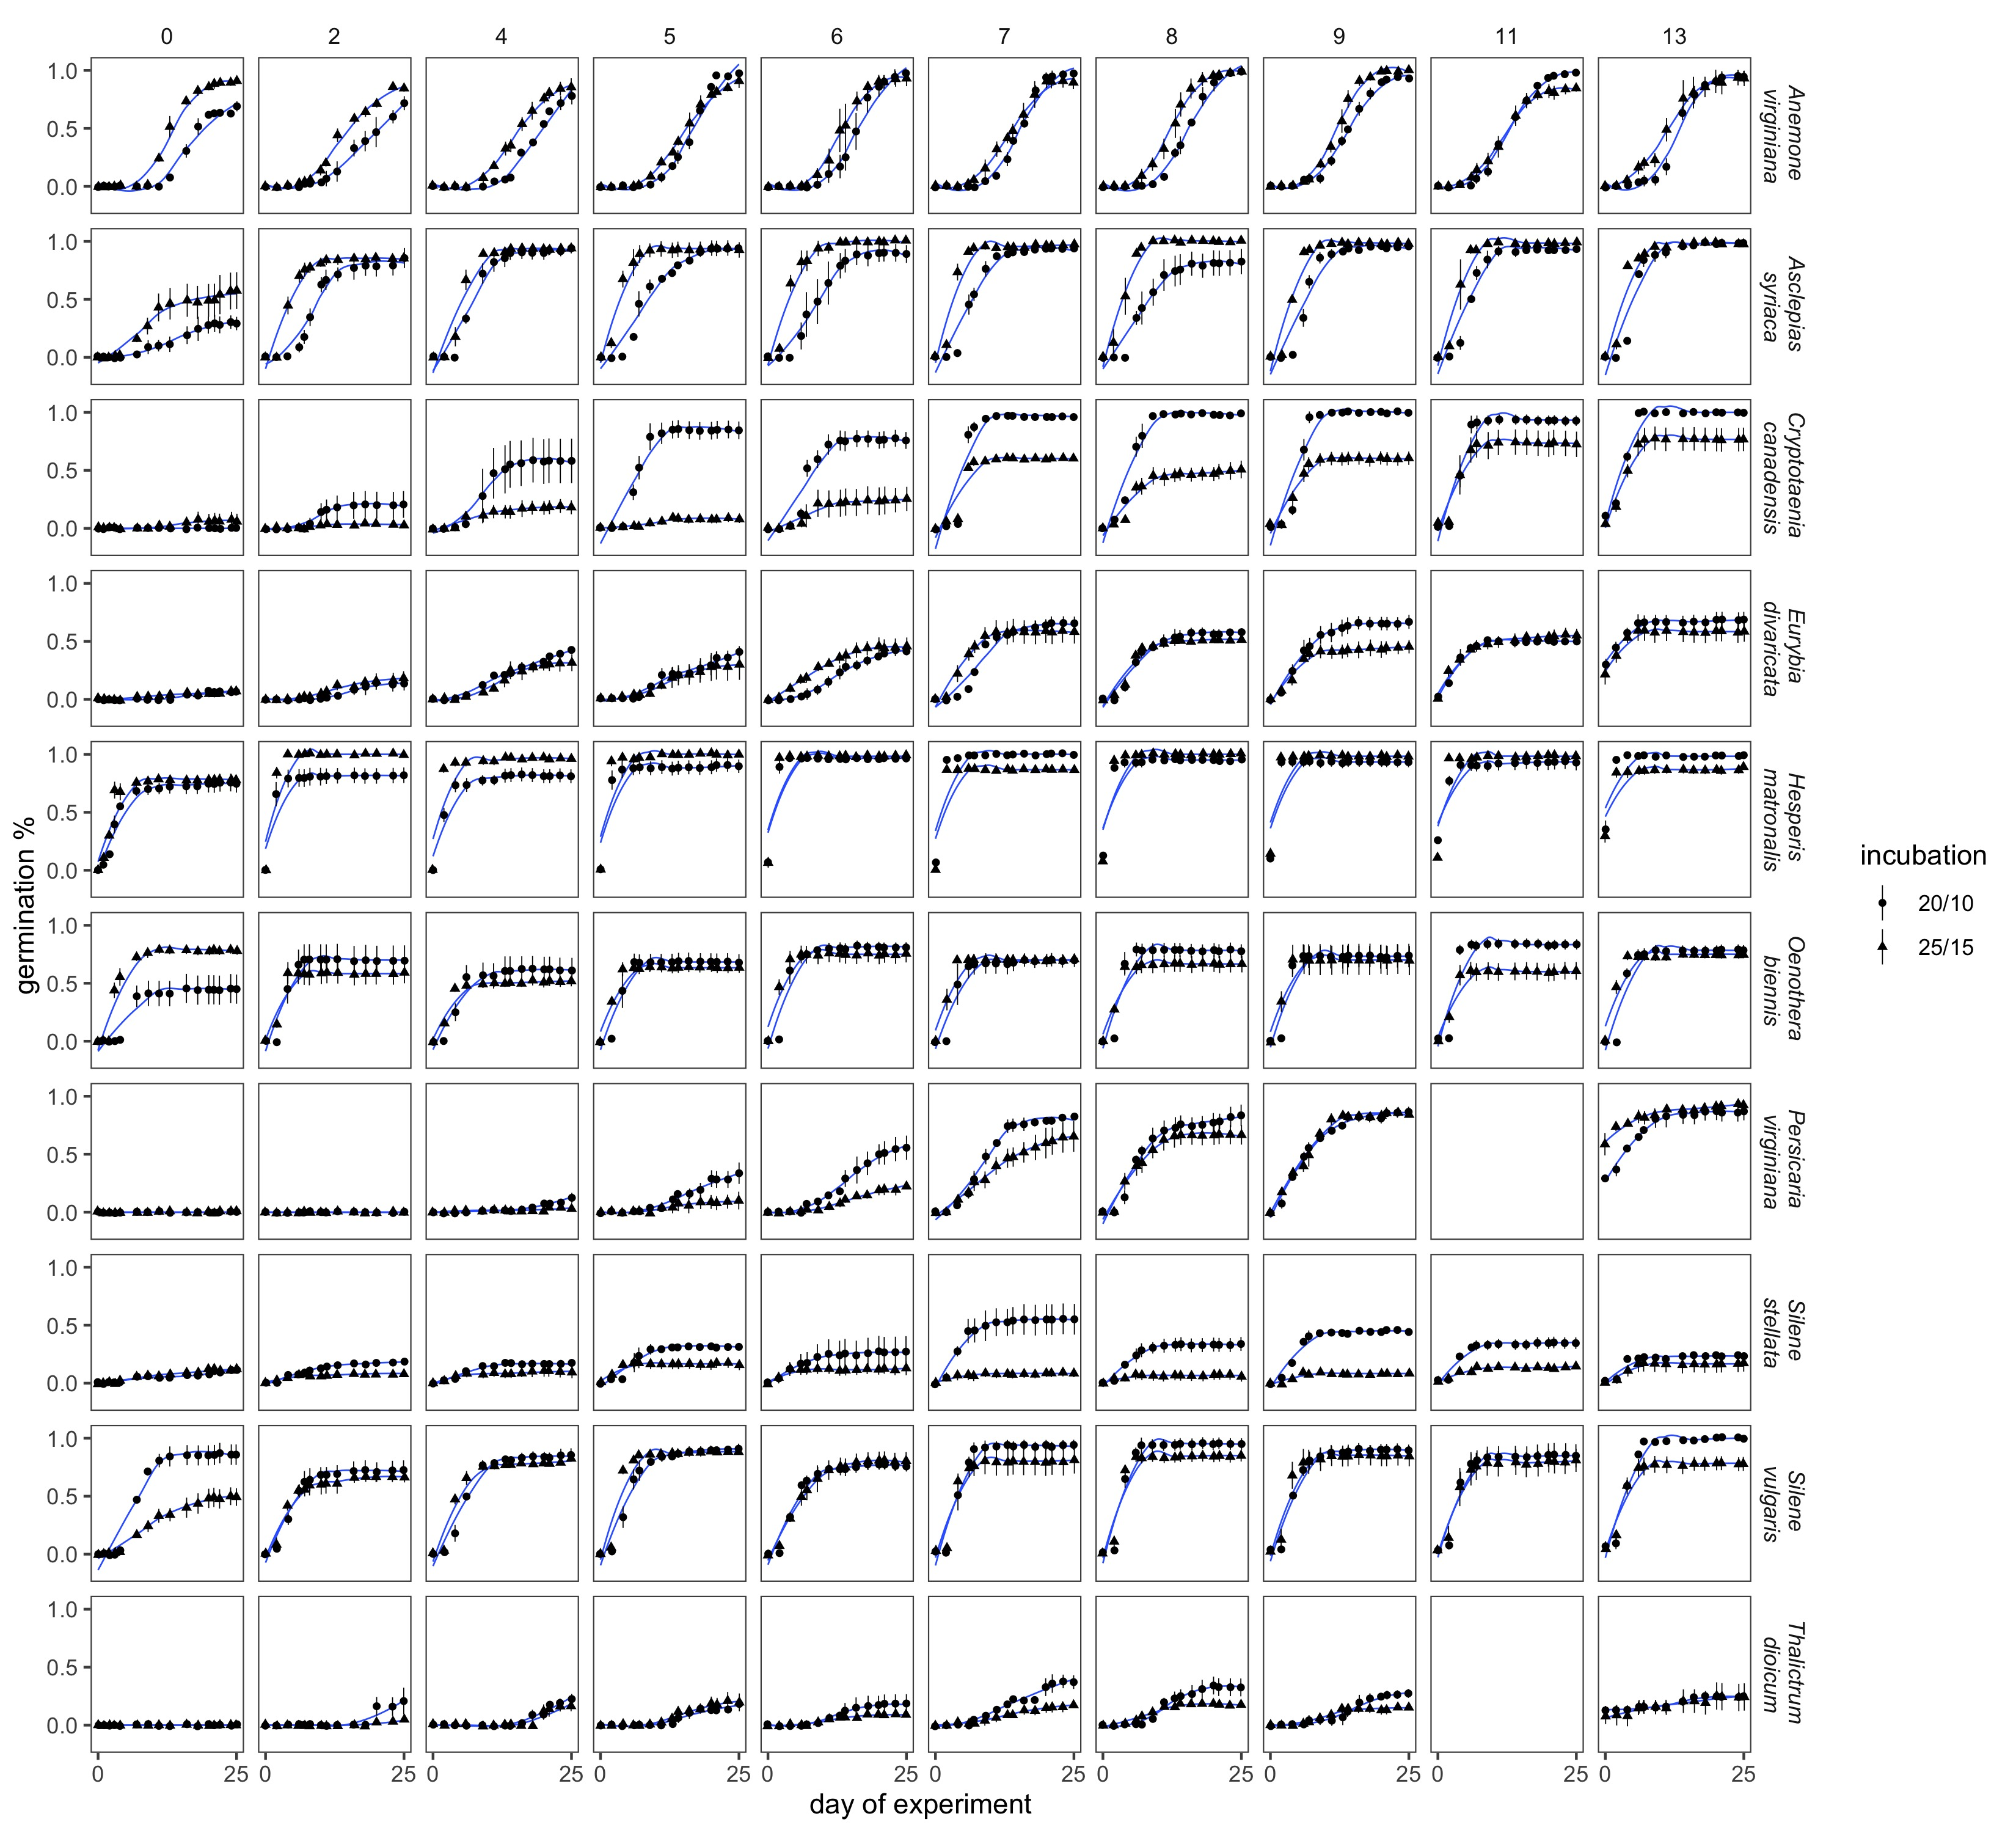
\includegraphics[width=\textwidth]{..//plots/germ_courses.jpeg}
    \caption{alternate empirical plot style?}
    \label{Fig:emp2}
\end{figure}

\begin{figure}[h!]
  \centering
 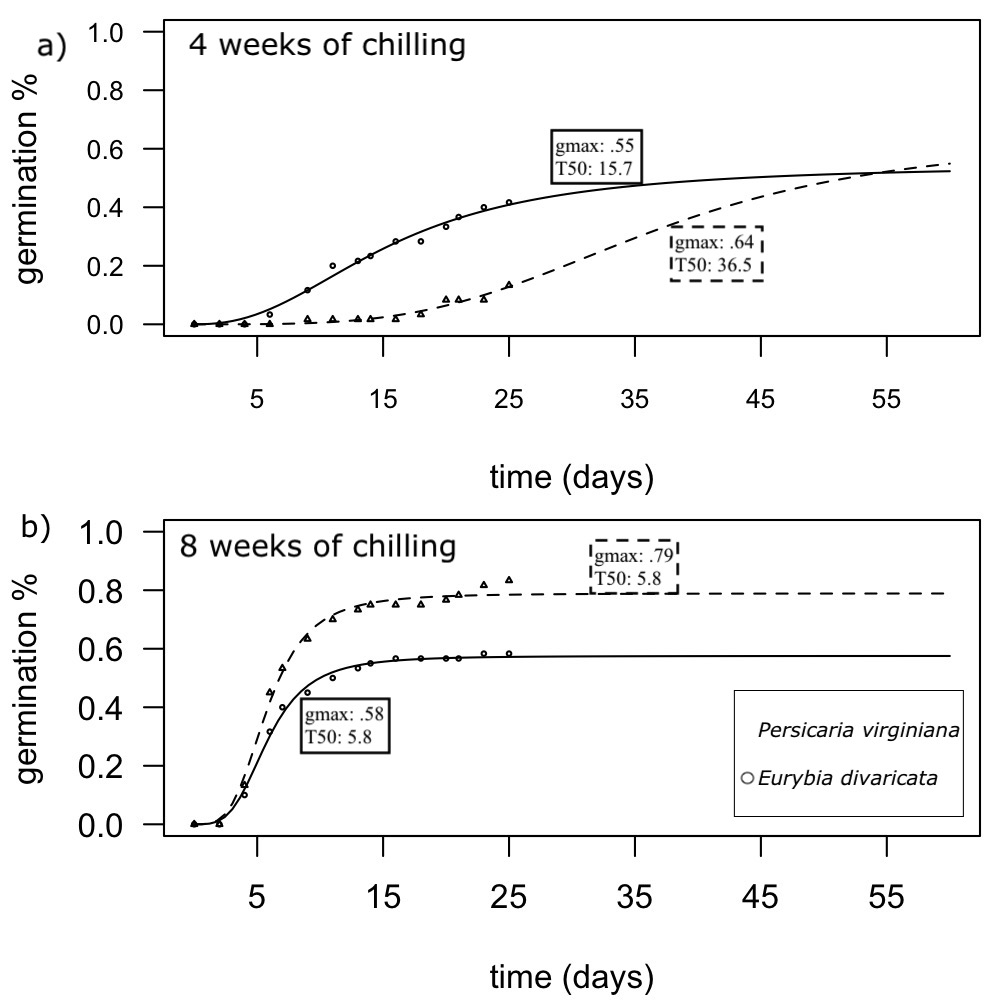
\includegraphics[width=\textwidth]{..//plots/examp_Ed_andPv.jpeg}
    \caption{case study to ease in drcs and highlight the compex relationship between time and fraction}
    \label{Fig:case}
\end{figure}


\begin{figure}[h!]
  \centering
 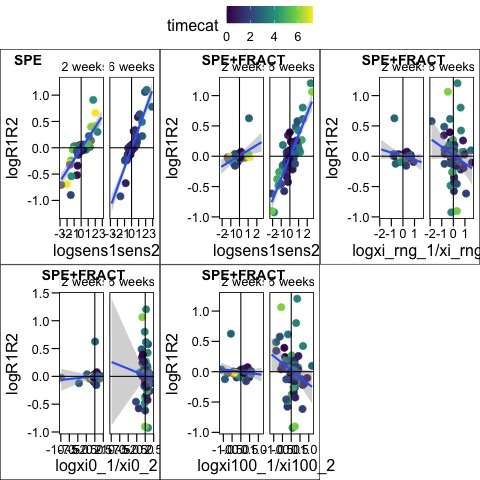
\includegraphics[width=\textwidth]{..//plots/coexistance_runner.jpeg}
    \caption{4\% of high chill cases result in coexistence and 3\% of low chill cases. The slope gets steeper in low chill scenario. Overall pretty limited change to coexistence overall, you just need more exteme differences in sensitivity to acheive it. Does this mean we need to tune the parameters?}
    \label{Fig:coexistence}
\end{figure}


\begin{figure}[h!]
  \centering
 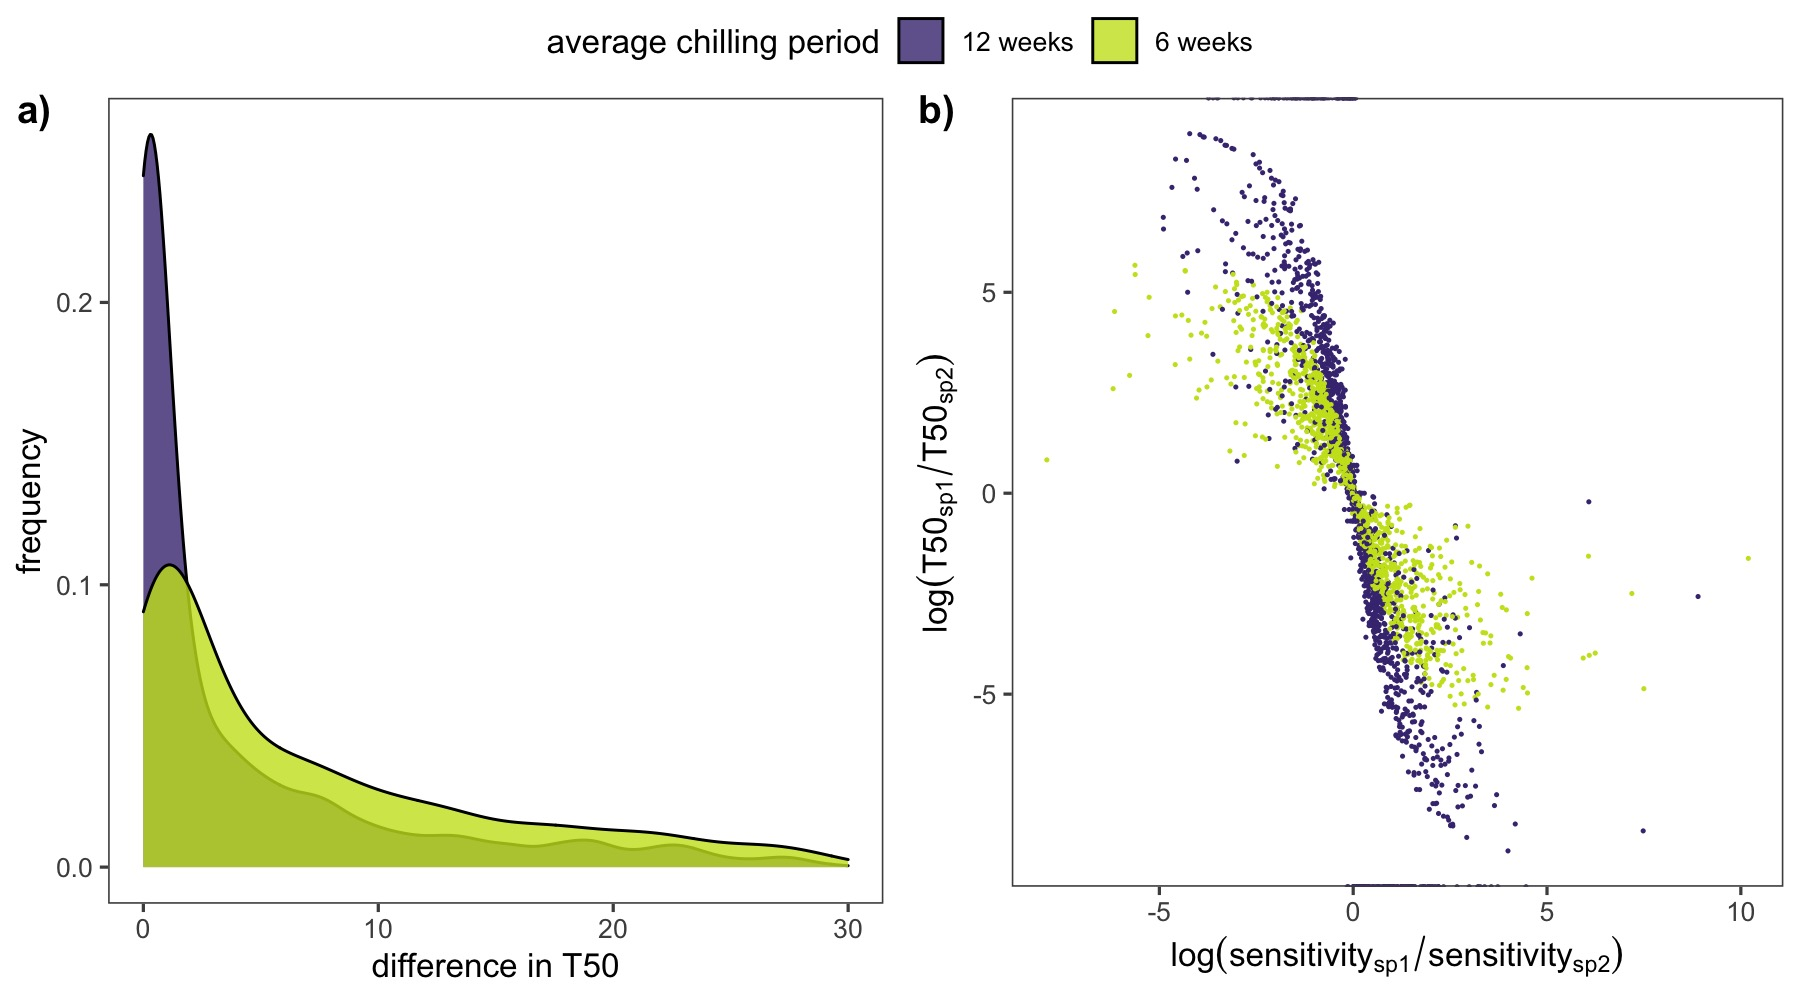
\includegraphics[width=\textwidth]{..//plots/coexistance_chilldiffs.jpeg}
    \caption{The mean difference in germination is lower with high chill (a). The same differences in sensitivity manifest in larger differences in germination time under high chill, so smaller differences in sensisitivity are more likely to lead to coexistence}
    \label{Fig:differences}
\end{figure}

\begin{figure}[h!]
  \centering
 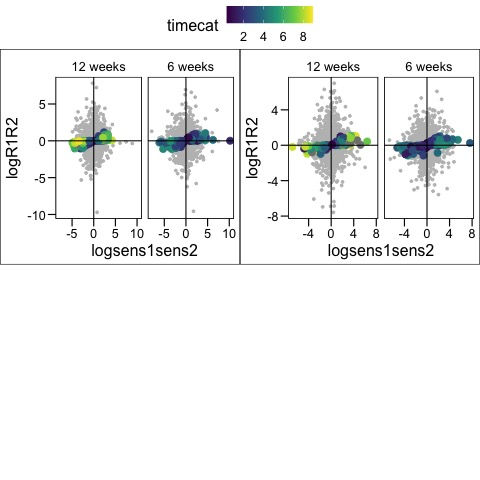
\includegraphics[width=\textwidth]{..//plots/dominance.jpeg}
    \caption{Not sure if we want to go down this path, but I also looked at scenarios where the worse competitor wins due to priority effects. This becomes more common in lower chilling world (180 cases vs 110 cases or 12\% of cases of competitive exclusion vs. 7\%). Suggesting (maybe) SPE's will play a strong role in compeition under warming?}
    \label{Fig:differences}
\end{figure}

\end{document}
